\chapter{Search for the decay %
  \texorpdfstring{$\boldsymbol{\btodsphi}$}{\btodsphi}}
\label{ch:dsphi}

This chapter describes the search for the decay \btodsphi, the results of which were published in
\Ref{PAPER}.

\section{Introduction}

\begin{figure}[bh]
  \begin{center}
    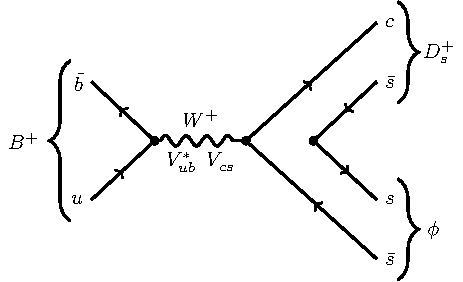
\includegraphics[scale=1]{feynman_dsphi_sm}
    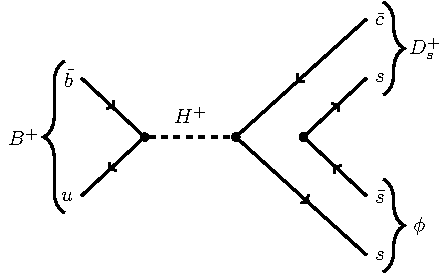
\includegraphics[scale=1]{feynman_dsphi_susy}
    \caption[Feynman diagram for the decay \btodsphi]
    {
      A Feynman diagram for the decay \btodsphi being mediated by a
      (left) \Wp in the SM, and
      (right) $H^+$ in SUSY.
      The \ssbar pairs shown here are formed from a gluon that can come from any quark.
      The arrangement of quarks forming the final state mesons shown is the colour favoured decay
    }
    \label{fig:dsphi:feyn}
  \end{center}
\end{figure}

In the \sm, the decay \btodsphi proceeds via the annihilation of the constituent \bquark and \uquark
quarks of a \Bp meson
forming a virtual \Wp boson from the \gls{CC} interaction, the processes is suppressed by the \ckm
matrix element \V{ub}\footnote{
  All mentions of the \phii meson refer to the $\phi(1020)$.
}.
To achieve the final state, the \Wp decays into a $\cquark\squarkbar$ pair and an additional
\ssbar pair must be created from the \QCD field.
This is the only diagram that can perpetuate such a decay at tree-level, because the initial state
quarks are all different to those in the final state.
A Feynman diagram of the decay \btodsphi is shown in \Fig{fig:dsphi:feyn}, where
the final state mesons can be formed in the way indicated, or the \ssbar pair from the \QCD field
can form the \phii, although this is colour-suppressed.
Also, the gluon that forms the \ssbar pair can originate from any of the initial or final state
quarks.
This analysis was published in \Ref{LHCb-PAPER-2012-025}.

Annihilation decays of \Bp mesons are rare in the SM due to the magnitude of
$|\V{ub}|\sim4\e{-3}$.
In fact, no fully hadronic decays proceeding via annihilation-type diagrams have yet been
observed.




%and SUSY, where the \ssbar pair are produced by a decaying gluon which could have
%originated from any of the four quarks.
%If the gluon were to be from one of the initial state quarks then the assumption of factorisation
%does not hold.

Predictions for the branching fraction $\BF\big(\btodsphi\big)$ are calculated using the OPE defined
by the effective Hamiltonian~\cite{Zou:2009zza,Mohanta:2002wf,PhysRevD.76.057701,Lu:2001yz}:
\begin{equation}
  \Ham{eff}=
  -4\frac{G_F}{\sqrt{2}} \V{ub}\Vconj{cs}
  \big[
    C_1(\Lambda)\Op{1}+C_2(\Lambda)\Op{2}
    \big]
\end{equation}
where
\begin{align}
  \Op{1} &= \big(\bquarkbar\gamma_\mu P_Lu\big) \big(\cquarkbar\gamma_\mu P_Ls\big) \nonumber\\
  \Op{2} &= \big(\bquarkbar\gamma_\mu P_Ls\big) \big(\cquarkbar\gamma_\mu P_Lu\big).
\end{align}
The Wilson coefficients $C_1$ and $C_2$ are defined at the scale $\Lambda=m_b$,
and the projection operators are defined as $P_L=\tfrac12(1-\gamma_5)$ and
$P_R=\tfrac12(1+\gamma_5)$.
The short distance operators \Op{1} and \Op{2} both describe the transition $b\!\to scu$.
Therefore, not only is there uncertainty in the branching fraction introduced by \V{ub}, but the
number of quarks in the decay make \QCD calculations very difficult.
Calculating the amplitude of the decay \btodsphi is made particularly complicated because the decay
is inherently non-factorizable, since the \ssbar pair can come from any of the initial or final
state quarks at leading order.
There are also inherent uncertainties in the form-factors that describe the hadronization
process of the final state quarks.
Reference~\cite{Mohanta:2002wf} predicts that
\begin{equation}
  \BF\big(\btodsphi\big)|{\makebox[\widthof{$_\mathrm{2HDM}$}][l]{$_\mathrm{SM}$}}
  =1.88\e{-6}, \nonumber\\
\end{equation}
by na\"ively assuming factorizability holds, and by using an improved
technique~\cite{Beneke:2000ry}, whereby perturbative \QCD corrections are applied to \added{the}
factorisation method, a value of
\begin{equation}
  \BF\big(\btodsphi\big)|{\makebox[\widthof{$_\mathrm{2HDM}$}][l]{$_\mathrm{SM}$}}
  =0.67\e{-6}, \nonumber\\
\end{equation}
is calculated.
\replaced{
The \QCD corrections lead to a new branching fraction prediction which differs by a factor of two
to the uncorrected result --- this is arguably testament to the difficulties of accounting for \QCD
in such calculations.
}{
The corrections lead to a factor two in the prediction of the branching fraction.
}
Other \sm predictions tend to lie between
\approx$1\e{-7}$ and
\approx$7\e{-7}$~\cite{Zou:2009zza,Mohanta:2002wf,PhysRevD.76.057701,Lu:2001yz}.

Despite the theoretical uncertainties, \deleted{enhancements in} the value of
in $\BF(\btodsphi)$ could be significantly enhanced if
the decay to be mediated by additional \bsm
particles, particularly other charged bosons.
For example, \replaced{a}{in a model with} \twoHDM --- such as \SUSY --- the decay \btodsphi
would be mediated by a charged Higgs $H^+$; this is shown in \Fig{fig:dsphi:feyn}.
More particles mean more Feynman diagrams that could add to the total amplitude.
Reference~\cite{Mohanta:2002wf} also makes predictions for the branching fraction of the decay
\btodsphi in a \twoHDM and a model with \rpv:
\begin{align}
  %\BF\big(\btodsphi\big)|{\makebox[\widthof{$_\mathrm{2HDM}$}][l]{$_\mathrm{SM}$}}
  %&=0.67\e{-6}, \nonumber\\
  \BF\big(\btodsphi\big)|_\mathrm{2HDM}
  &=8.0\pz\e{-6}, \nonumber\\
  \BF\big(\btodsphi\big)|{\makebox[\widthof{$_\mathrm{2HDM}$}][l]{$_\mathrm{RPV}$}}
  &=3.06\e{-4}. \nonumber
\end{align}
%The above number for the \sm branching fraction was calculated using the \QCD improved
%factorization method~\cite{Beneke:2000ry}, but to illustrate the difficulties in \QCD calculations,
%the same paper quotes $1.88\e{-6}$ using the factorization approximation.
These numbers indicate that, while the exact \sm value of $\BF\big(\btodsphi\big)$ is not well
known, the value for models with additional mediating particles could be enhanced by a factor of
over 100.

The \CP asymmetry, \acp, of a process is defined in terms of decay rates of $B$ hadrons:
\begin{equation}
  \acp = \frac{\Gamma(\Bbar\!\to\xbar{f}) - \Gamma(B\!\to f)}
  {\Gamma(\Bbar\!\to\xbar{f}) + \Gamma(B\!\to f)}
\end{equation}
for some final state $f$.
A positive value of \acp would indicate a preference of the antimatter process, above the matter
process.
In the \sm $\acp(\btodsphi)=0$, because
\replaced{
  at leading order there is only one phase, in \V{ub}
}{
  the process only contains one phase, in \V{ub}
}, but
interference from \bsm physics diagrams could alter this significantly.
Predictions from \Ref{Mohanta:2002wf} are:
\begin{align}
  \acp\big(\btodsphi\big)|_\mathrm{2HDM}
  &\leq 59\,\%, \nonumber\\
  \acp\big(\btodsphi\big)|{\makebox[\widthof{$_\mathrm{2HDM}$}][l]{$_\mathrm{RPV}$}}
  &\leq 14\,\%.
  \label{eq:dsphi:acpdef}
\end{align}
So, both measurements of $\BF\big(\btodsphi\big)$ and $\acp\big(\btodsphi\big)$ could lead to
evidence for \np.


\subsection{Other annihilation-type hadronic decays}
The annihilation of the \Bp meson can perpetuate numerous decays resulting in fully hadronic
states, including a charmed meson.
The decay \decay{\Bp}{\Dp\Kstarz} proceeds in the same way as
\btodsphi, but the former needs a \ddbar pair to be created from the \QCD vacuum, rather than an
\ssbar pair.
Similarly, the decay \decay{\Bp}{\Ds\Kstarzb} is identical to the \btodsphi excepting that instead
of \decay{\Wp}{\cquark\squarkbar} the \Wp decays into an $\cquark\dquarkbar$ pair.
The decays \decay{\Bp}{\Dp\Kstarzb} and \decay{\Bp}{\Ds\Kstarz} are non-trivial diagrams in the
\sm, and heavily suppressed, but have similar final states.
The same final states can also come from the annihilation of the constituent
quarks of the \Bc meson.
While the following chapter only discusses the search for the decay \btodsphi, these other
interesting decay modes are searched for in
\Ref{LHCb-PAPER-2012-025}.







\section{Data selection}
\label{sec:dsphi:sel}

%LIST
%
%Rely on HLT2 tolo lines
%cuts designed to mimic HLT1 and HL2 topo triggers:
%B
%sum pt $>$ 5\gev
%VHI2DOF $<$ 10
%BPVIPCHI2 $<$25
%BPVLTIME$>$0.2\ps
%BIRA$>$0.999
%
%D
%sum PT $>$1.8GeV
%MAXDOCA$<$0.5mm
%VCHI2DOF $<$10
%BPVVDCHI2$>$36
%
%D tracks
%TRCHI2<4
%PT>100MeV
%P>1Gev
%MIPCHI2>4
%DLL<20-10)
%
%phi
%sumPT>1
%VCHI2DOF<16
%BPVVDCHI2>16
%
%phi tracks
%TRCHI2<4
%PT>100MeV
%P>2GEv
%DLL<20-10)
%
%Min one track \& two...


The data sample used in this analysis amounts to
$1\invfb$ of $pp$ collisions at $7\tev$ collected by the \lhcb detector in 2011.
Events are selected by the trigger at hardware level if they fulfill the requirements of the \lone
hadron trigger, or any track in the event fulfills any \lone trigger line requirement (\tis).
Further trigger requirements are applied at the \hlttwo level, where events are required to pass at
least one of the hadronic topological triggers (see \Sec{sec:lhcb:trig} for more details) with
\tos.

The \Ds meson is only reconstructed from the Cabibbo favoured decay \dstokkpi,
which has a branching fraction of $(5.39\pm0.21)\e{-2}$.
Furthermore, the mass of the reconstructed particle must fall within $25\mev$ of
$m_{\Ds}^\pdg=1968.30\pm0.11\mev$; where the superscript \pdg indicates the nominal mass of the
indicated particle from \Ref{PDG2012}.
The \Ds meson decays weakly, and therefore has a non-zero lifetime,
$\tau_{\Ds}=(5.00\pm0.07)\e{-13}$, and thus an extremely narrow width, so the value of $25\mev$
is primarily to account for detector resolution effects.
In order for the candidate to have the correct decay topology, it is also required that the \Ds
vertex lies downstream of the \Bp decay vertex.

Candidate \phii mesons are reconstructed from the decay mode \phitokk, where
$\BF(\phitokk)=(0.498\pm0.005)$ and are accepted if the
invariant \kk mass, $\mass{\kk}$, is within $40\mev$ of
$\mass{\phi}^\pdg=(1019.461\pm0.019)\mev$~\cite{PDG2012}.
The \phii meson decays strongly, and therefore has an appreciable width,
$\Gamma_\phi=(4.266\pm0.031)\mev$, but the detector resolution is better for the \phii than the \Ds
because of it has zero lifetime.
Therefore, a mass window of $40\mev$ is extremely wide; but further mass constraints of the \phii
are applied in the signal yield fit, such that the signal region is defined by a window that
extends only $20\mev$ from $\mass{\phi}^\pdg$.

All tracks forming the candidate mesons must fulfill requirements on the transverse momentum,
$\pt>100\mev$, and tracks from the \Ds(\phii), $p>1(2)\gev$.
Geometrical constraints are also placed on the tracks.
The \chisq per degree of freedom of the track fit, $\chisqtrk/\ndof$, must be less than four, and
$\min\left(\chisqip\right)>4$.
The variable \chisqip is defined as the increase in the \chisq of the vertex fit (\chisqvtx) when
the signal track is combined with the PV; the $\min\left(\chisqip\right)$ is the minimum \chisqip
with respect to all PVs.
Loose PID requirements are also placed on all tracks, and further PID constraints are applied in
the \bdt, which is detailed later.

The \Bp vertex fit is performed by constraining the mass of the \Ds to its known
mass~\cite{PDG2012}, and the resulting vertex fit must have a \chisqvtx per degree of freedom of
less than ten.
A requirement of $\cos\thetadir>0.999$ must also be met.
The angle \thetadir is defined as the angle between the momentum vector of the \Bp candidate and
the vector formed by the PV and decay vertex of the \Bp.
Were the resolution of the \lhcb detector to be perfect, a real decay would have $\cos\thetadir=1$.
Prompt background from the PV is suppressed by requiring that the lifetime of the \Bp,
$\tau_{\Bp}$, is greater than $0.2\ps$.
Cuts applied in the stripping are summarized in \Tab{tab:dsphi:sel}.


%Candidate \Ds and \phii mesons are reconstructed only in the decays \decay{\Ds}{\kkpi} and
%\phitokk, where the \Ds decay is the Cabibbo favoured mode.
%Each daughter track has a $\chisqtrk/\ndof<4$, a \pt of at least $100\mev$, and a minimum momentum
%of $1$ or $2\gev$ for tracks originating from the \Ds and \phii, respectively.
%Each track in the event must also be detached from the PV, and are only accepted if the
%$\chisqvtx/\ndof$ increases by more than four when the track is used in the vertex fit, compared to
%when it is omitted.
%Very loose PID requirements are also placed on the tracks, this is more to reduce the rate of the
%stripping line that to identify pions and kaons, this is done later in the selection process.

%The \Ds and \phii are also subject to requirements on the \chisq of the vertex separation,
%\chisqvs, which is tighter for the \Ds because of its finite lifetime.
%Full stripping requirements are given in \Tab{tab:dsphi:sel}.

\begin{table}[!ht]
  \caption[Selection requirements of \btodsphi candidates]
  {
    Selection applied to the \btodsphi candidates.
    The DOCA variable is defined as the maximum distance of closest approach between all pairs of
    all pairs of daughter particles.
    All remaining variables are defined in the text.
  }
  \label{tab:dsphi:sel}
  \begin{center}
    \begin{tabular}{llcrc}
      \toprule
      Candidate & \multicolumn{4}{c}{Selection requirement} \\
      \midrule
      \Bp
      %\multirow{5}{*}{\Bp}
      & $\sum p_T^\mathrm{tracks}$ &$>$& $5$ & GeV \\
      & \chisqvtx/\ndof &$<$& 10 \\
      & \chisqip &$<$& 25 \\
      & $\tau$ &$>$& $0.2$ & ps \\
      & $\cos\thetadir$ &$>$& $0.999$ \\
      %& $\bdt_\mathrm{strip}$ &$>$& 0.05 \\
      \littlerule
      \Ds
      %\multirow{3}{*}{\Ds}
      & $\sum p_T^\mathrm{tracks}$ &$>$& $1.8$ & GeV \\
      & \chisqvtx/\ndof &$<$& 10 \\
      & DOCA &$<$& $0.5$ & mm \\
      \littlerule
      Tracks from \Ds
      %\multirow{6}{*}{Tracks from \Ds}
      & \pt &$>$& $100$ & MeV \\
      & $p$ &$>$& $1$  & GeV\\
      & $\chisqtrk/\ndof$ &$<$& $4$ \\
      & $\min\!\left(\chisqip\right)$ &$>$& $4$ \\
      & \chisqfd &$>$& 36 \\
      & $\dllkpi(K)$ &$>$& $-10$ \\
      & $\dllkpi(\pi)$ &$<$& $20$ \\
      \littlerule
      \phii
      %\multirow{2}{*}{$\phi$}
      & $\sum\pt^\mathrm{tracks}$ &$>$& 1&GeV   \\
      & \chisqvtx/\ndof &$<$& 16 \\
      \littlerule
      Tracks from $\phi$
      %\multirow{4}{*}{Tracks from $\phi$}
      & \pt &$>$& 100 & MeV \\
      & $p$ &$>$& 2 & GeV \\
      & $\chisqtrk/\ndof$ &$<$& $4$ \\
      & $\min\!\left(\chisqip\right)$ &$>$& $4$ \\
      & \chisqfd &$>$& 16 \\
      %\midrule
      %STUFF FOR 1 AND 2 TRACKS
      \bottomrule
    \end{tabular}
  \end{center}
\end{table}


%After the stripping selection, further cuts are applied.
%The invariant mass of the \Ds candidates are required to be within $25\mev$j
%its nominal value cited in \Ref{PDG2012}.
%Cuts are also applied to reconstructed \phii mass, this is described later, in \Sec{sec:dsphi:hel}.
%The decay vertex of the \Ds is required to be downstream of the decay vertex of the \Bp, and the
%$p$-value formed from the sum of the \chisqip and \chisqvtx of the \Bp candidate is also required
%to be greater than $0.1\pc$.
%Charmless backgrounds are suppressed by requiring that the \chisqfd from the \Bp vertex was greater
%than two.



%These peaking backgrounds do not necessarily result in a longitudilnally polarized \phii.
%They are however, irriducible, and must be accounted for in the fit, this is described later in
%\Sec{sec:dsphi:fit}.

%In order to remove candidates from \Dp cross-feed,
%if the new $\Km\pip\pip$ mass falls within $25\mev$ of $m_{\Dp}^\pdg$,
%the kaon pair must either form an invariant mass within
%$10\mev$ of the known \phii mass, or the ambiguous track must pass stringent PID requirements
%($\dllkpi(\Kp)>10$).
%If the mass of the $p\Km\pip$ object falls within $25\mev$ of the \Lc mass,
%The candidate decay chain is then subject to the stripping requirements, which are outlined in
%\Tab{tab:dsphi:sel}.
%Requirements in the stripping are that the \Ds vertex is downstream of the \Bp and the vertices are
%well defined.
%One variable listed in \Tab{tab:dsphi:sel} is $\bdt_\mathrm{strip}$, which is the output of a BBDT
%in the stripping, whose input variables are a few kinematic and geometric variables of the \Bp and
%\Ds.
%The cut on this BBDT is very loose, and is approximately 100\pc efficient
%The \decay{\Ds}{\kkpi} and \decay{\phi}{\kk} candidates are required to have invariant masses
%within 25 and $20\mev$ of their known masses~\cite{PDG2012} respectively.



\subsection{Suppression of combinatorial background}
A pair of \bdt{s} are employed to
separate \dstokkpi and \phitokk candidates from combinatorial background; referred to as
$\bdt_{\Ds}$ and $\bdt{\phi}$, respectively.
The \bdt{s} are designed to identify the
decays \dstokkpi and \phitokk, with topologies consistent with coming from a parent $B$-meson.
The methodology used to train each \bdt is the same.
Both are trained using the bagging algorithm using the same set of input variables.
This technique of using a \bdt to identify each meson is also used in
\Ref{LHCb-CONF-2012-009}, which measures branching fraction ratios of various \decay{B}{DD} decays.

%Each BDT was trained using the bagging method, as described in \Sec{sec:bdt:bag}.
%The signal and background data used to train these BDTs came entirely from data.
%Signal samples came from the decays $\decay{\Bbar^0_{s}{\Ds\pim}$ and $\decay{\Bs}{\jpsi\phi}$
%data, which was background subtracted by sWeighting~\cite{splot}.
%Background samples were taken from the sideband distributions of the same data.
%The BDT technique used in this analysis, also used in \Ref{LHCb-CONF-2012-009}, is different to
%other analyses in this thesis in that a BDT is trained for each the \Ds and $\phi$.

The \bdt trained to identify \dstokkpi was trained using a pure sample of \dstokkpi decays from the
high statistics channel \decay{\Bsb}{\Dsp\pim}.
The signal sample was background subtracted using the sWeighting technique~\cite{splot}, and the
background sample is taken from the mass sidebands of the \Ds meson.
Similarly, for the \phii \bdt, the signal sample was sWeighted and the background comes from the
\phii mass sidebands; but the sample is taken from the high statistics \bstojpsiphi mode.

Considering that each \bdt was trained on data, variables that are poorly described in simulation
can be used in the training.
In total, there are five kinematic and geometric training variables for the parent meson.
For the daughter tracks there are a total of 23 variables, including kinematic, geometric and \pid
variables.
A summary of all training variables is given in \Tab{tab:dsphi:vars}.


%The BDT used to separate background from the signal \decay{\Ds}{\kkpi} decays was trained using
%a signal sample of \decay{\Bs}{\Dsm\pip} sWeighted~\cite{splot} data, and background from the \Dsm
%sidebands.
%This BDT uses an unusually large array of training variables, given in \Tab{tab:dsphi:vars},
%which include PID, and track quality variables.




\begin{table}
  \caption[BDT variables]
  {
    List of training variables used in the \Ds and \phii BDTs.
    Each BDT uses five variables associated with the parent particle and 23 variables from each
    daughter track.
  }
  \label{tab:dsphi:vars}
  \begin{center}
    \begin{tabular}{clp{0.50\textwidth}}
      \toprule
      Particle & \multicolumn{2}{c}{Variable} \\
      \midrule
      \Ds, \phii
      & Kinematic variables & $p$, \pt \\
      & Geometric variables & \chisqvtx, \chisqip, \chisqfd \\
      \littlerule
      Tracks
      & Kinematic variables & $p$, \pt \\
      & Geometric variables & $\min(\chisqip)$ \\
      & Track variables     & 4 variables characterizing the track quality \\
      & PID variables       & 16 variables containing PID information, such as {\tt isMuon} and DLL
      variables from the \rich detectors \\
      \bottomrule
    \end{tabular}
  \end{center}
\end{table}


The cut for the \bdt was optimized using the metric $S/\sqrt{S+B}$,
In this case, the number of signal events, $S$, was estimated from the yield from the decay
\decay{\Bs}{\Dsm\pip}, according to:
\begin{equation}
  S = \frac{ \BF\big(\btodsphi\big) }{ \BF\big(\Bsb\!\to\Ds\pim\big) }
  \frac{ \eff{gen}\big(\btodsphi\big) }{ \eff{gen}\big(\Bsb\!\to\Ds\pim\big) }
  \frac{f_d}{f_s}
  N\big(\Bsb\!\to\Ds\pim\big),
\end{equation}
$f_s/f_d$ quantifies the fraction of \Bs mesons produced relative to \Bd mesons.
The generator level efficiency, \eff{gen}, is the efficiency introduced by the acceptance region of
the \lhcb, and the necessity that all daughter particles must travel through the detector.
Background yield for a given cut is estimated as:
\begin{equation}
  B = c\cdot N_\mathrm{c}\big(\bstodspi\big)\cdot N_\mathrm{c}\big(\bstojpsiphi\big),
\end{equation}
where $N_\mathrm{c}$ indicates the yield of the combinatoric background for the indicated decay,
and $c$ is a constant scaled such that $N_\mathrm{c}\big(\bstodspi\big)\cdot
N_\mathrm{c}\big(\bstojpsiphi\big)=N_\mathrm{c}\big(\btodsphi\big)$ with no \bdt cut.
The optimization procedure results in the optimal cut as $\bdt_{\Ds}\times\bdt_\phi>0.57$, as is
shown in \Fig{fig:dsphi:opt}.


\begin{figure}
  \begin{center}
    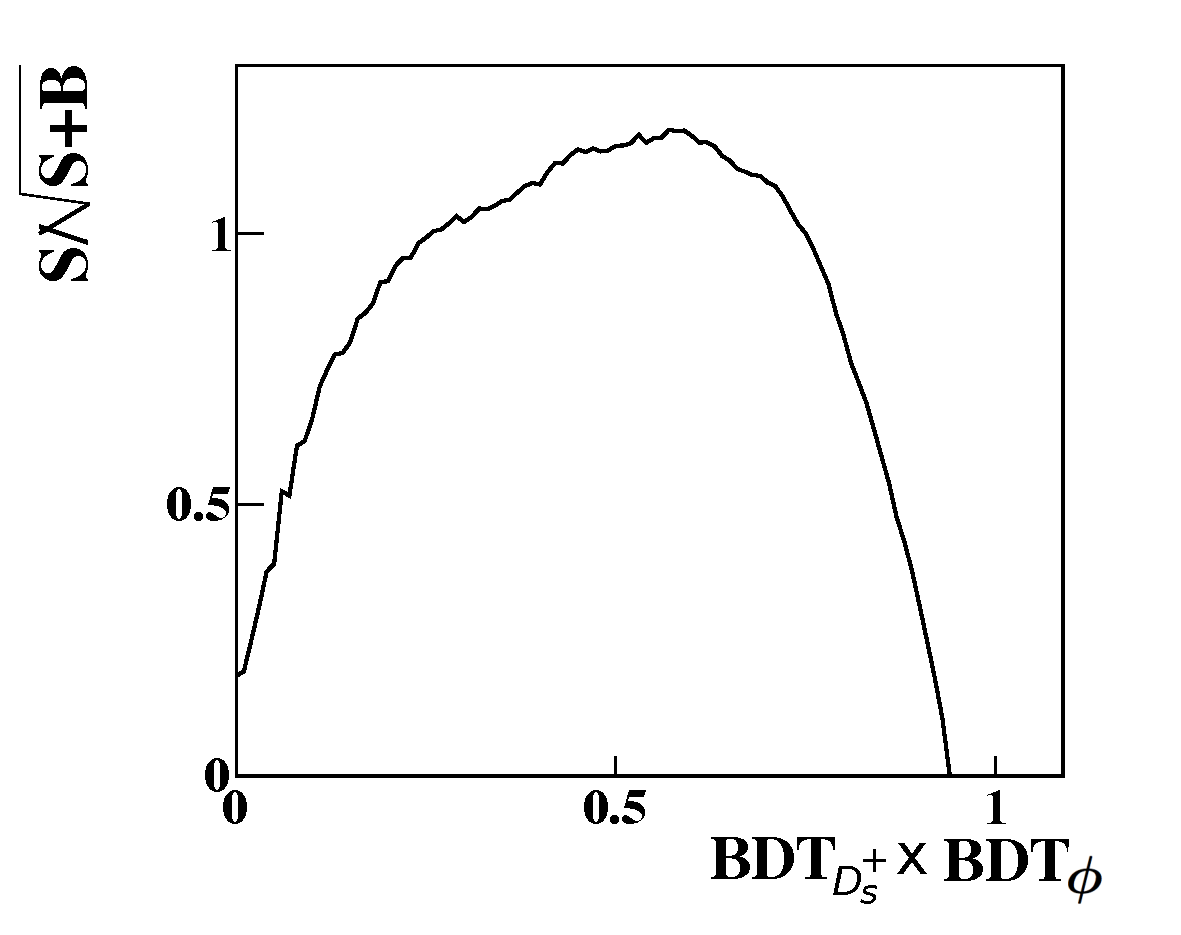
\includegraphics[width=0.48\textwidth]{dsphi_opt}
    \caption[Optimization of BDT cut for selection of \btodsphi candidates]
    {
      Value of the figure of merit $S/\sqrt{S+B}$ is shown as a function of the \bdt response,
      $\bdt_{\Ds}\times\bdt_{\phi}$.
      The maximum value of the figure of merit is 0.57, which is chosen as the final \bdt cut.
    }
    \label{fig:dsphi:opt}
  \end{center}
\end{figure}


%The boosting technique used here was bagging, which --- as described in \Sec{sec:bdt:bag} --- gives
%a response in the range $0<\mathrm{BDT}<1$.
%Cutting on the product of the two BDT responses improves the performance, and therefore the cut is
%$\bdt_{\Ds}\times\bdt_\phi>X$, as opposed to $\bdt_{\Ds}>X_1$ and $\bdt_\phi>X_2$.



\subsection[Vetoes of contributions from the decays {\decay{\Dp}{\kpipiss}} and \decay{\Lc}{\pkpi}]
{Vetoes of contributions from the decays $\boldsymbol{\decay{\Dp}{\kpipiss}}$ and $\boldsymbol{\decay{\Lc}{\pkpi}}$}
There are few backgrounds from real particles that could contaminate the final selection after the
\bdt selection.
The decay topology of \dstokkpi is very similar to the other weak decays \decay{\Dp}{\kpipiss} and
\decay{\Lc}{\pkpi}.
These have relatively large branching fractions~\cite{PDG2012}:
\begin{align}
  \BF(\decay{\Dp}{\kpipiss}) &= (9.13\pm0.19)\e{-2} \\
  \BF(\decay{\Lc}{\pkpi}) &= (5.0\pm1.3)\e{-2},
\end{align}
and if the daughter \pip(\proton) from the \Dp(\Lc) decay is misidentified as a \Kp the decay
\dstokkpi can be mimicked.
%the resulting invariant mass combination can fall within $25\mev$ of \mass{\Ds}.
Henceforth, the notation $h_i$ will be used to denote a particle assigned the mass of an $h$ which
has been identified as an $i$.
Simple generator level simulations of phasespace illustrate that
the mass combination of $\Kp_\pi\Km\pip$ and $\Kp_p\Km\pip$ from a real \Dp or \Lc, respectively,
can fall within $25\mev$ of $\mass{\Ds}^\pdg$; as shown in \Fig{fig:dsphi:veto}.


\begin{figure}
  \begin{center}
    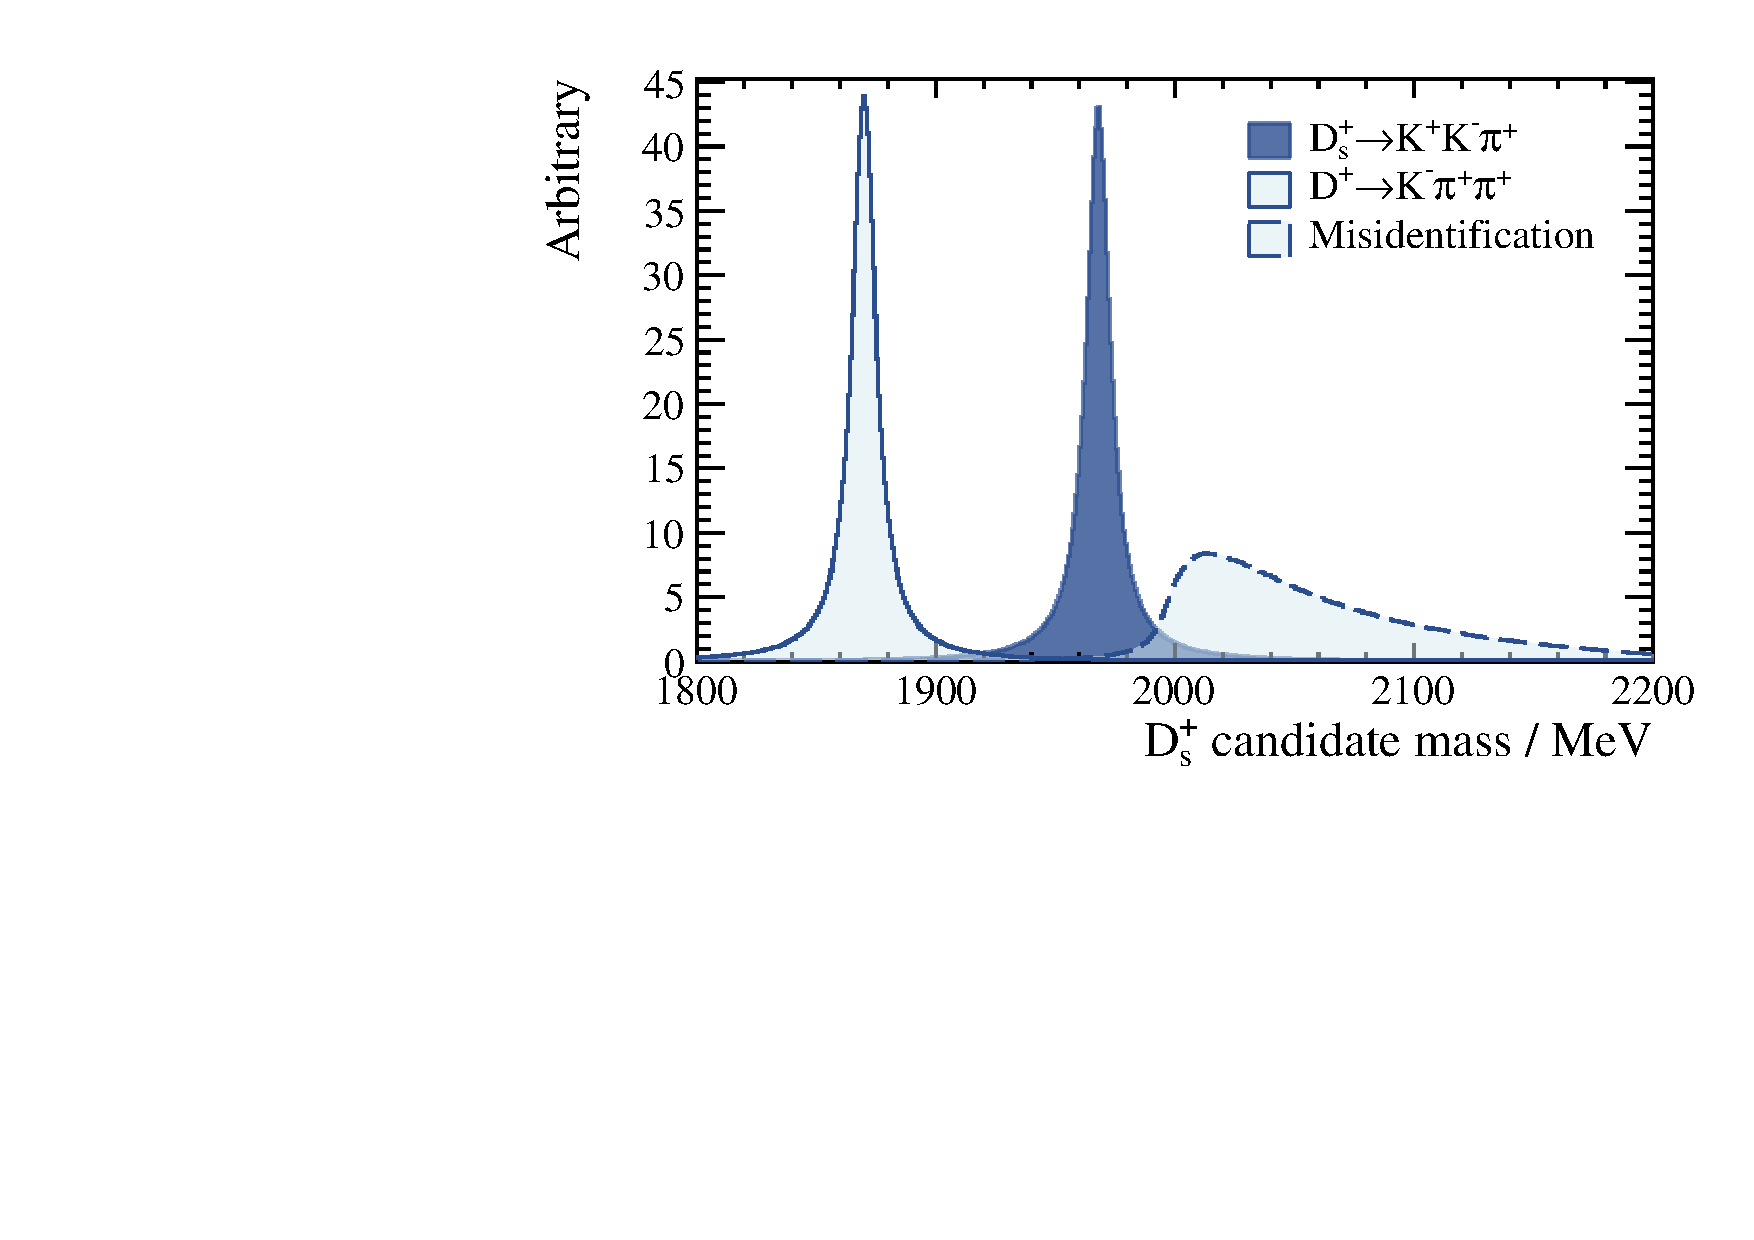
\includegraphics[width=0.48\textwidth]{tgen_dveto}
    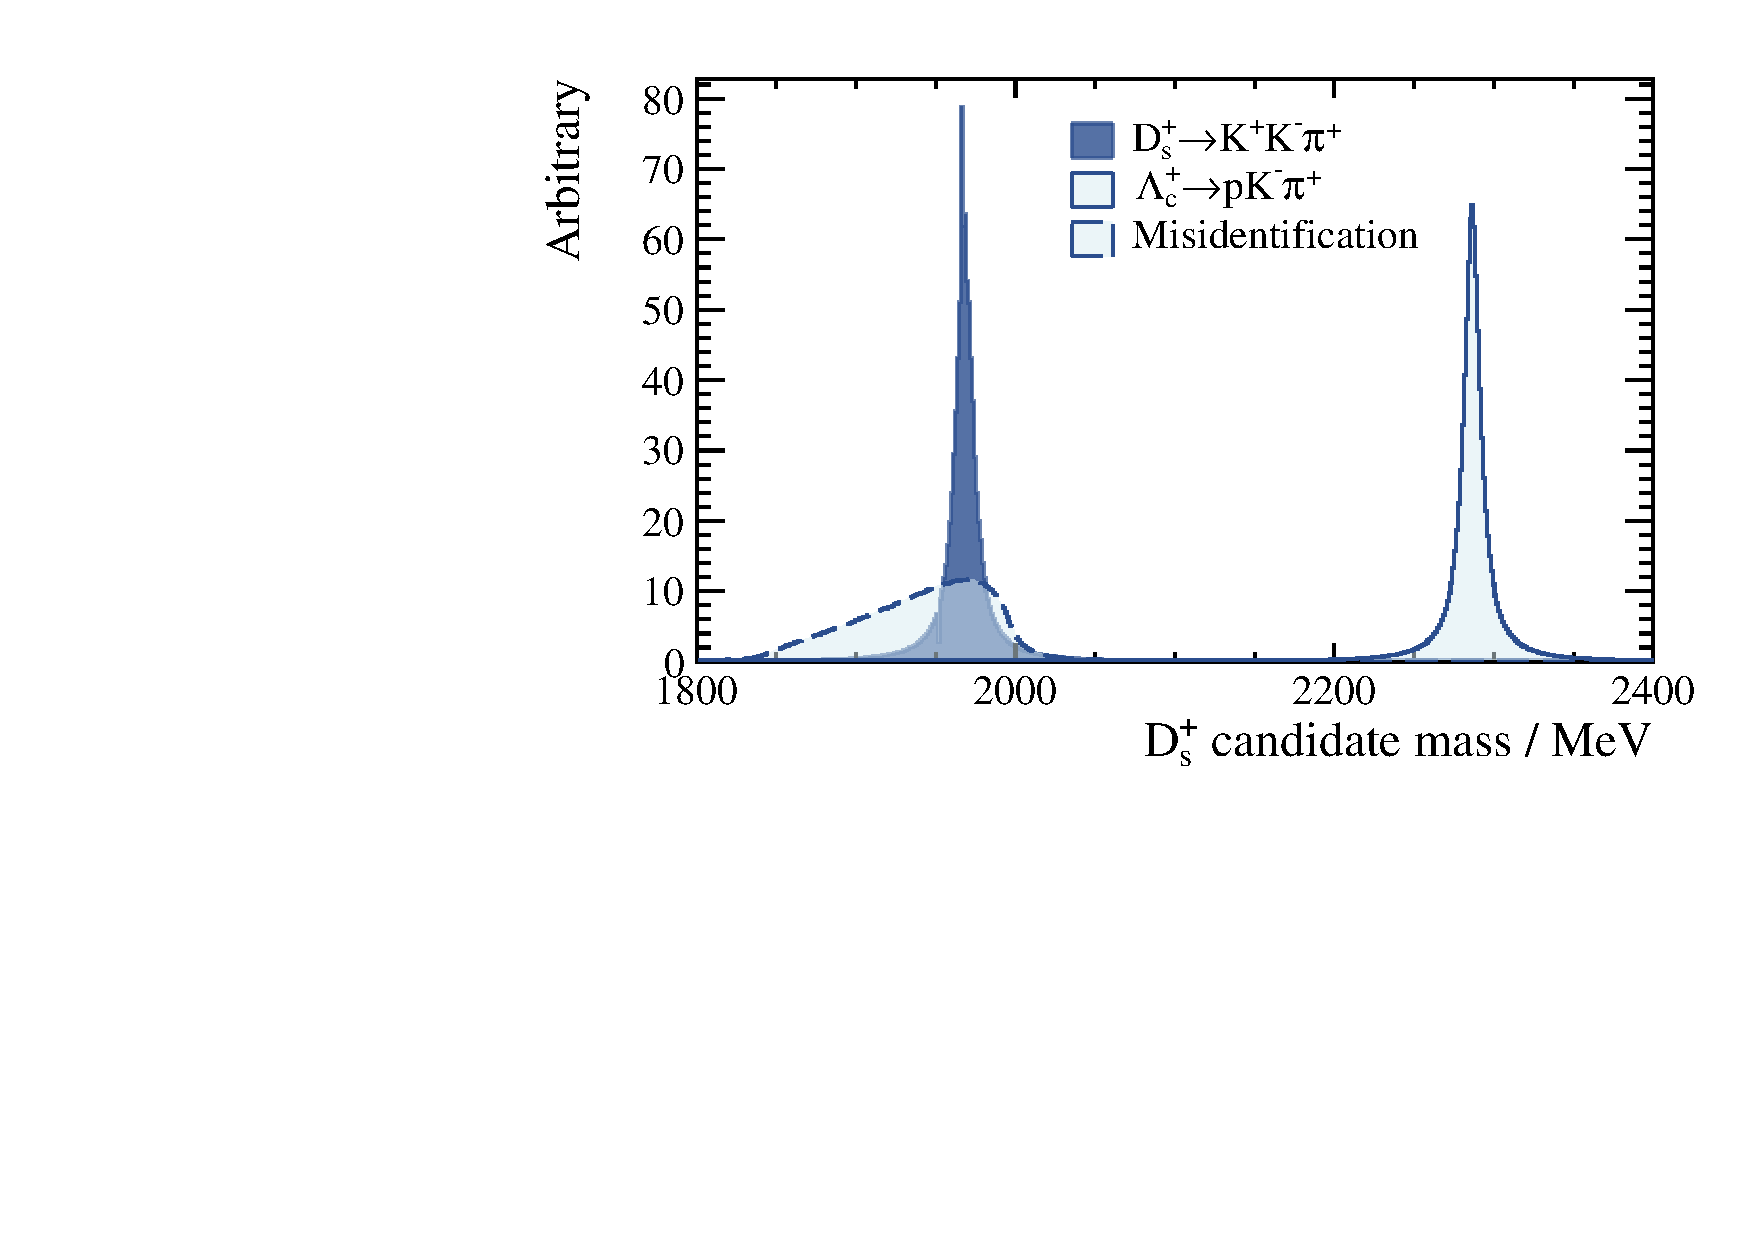
\includegraphics[width=0.48\textwidth]{tgen_lcveto}
    \caption[Vetoing \Ds contamination from \Lc and \Dp decays]
    {
      Simple phasespace simulations at generator level of the decay \decay{\Ds}{\kkpi}, along side
      (left) \decay{\Dp}{\kpipiss}, and
      (right) \decay{\Lc}{\pkpi},
      The distributions of the \Dp and \Lc decays, where one particle has been misidentified as a
      \Kp are also shown.
      Distributions after the misidentification are shown with a dotted outline, and sit under the
      \Ds mass peak.
      Magnitudes of each peak are meaningless, each having the same integral.
    }
    \label{fig:dsphi:veto}
  \end{center}
\end{figure}

The cross-feed from the \Dp and \Lc is suppressed by vetoes, whereby tight \pid constraints are
applied if the \dstokkpi candidate could have come from either a \Dp or \Lc.
Firstly, if the invariant mass of the \kk pair is lies within $10\mev$ of the nominal \phii mass
then it is highly likely that it is a real \Ds decaying via \decay{\Ds}{\phi\pip}, which has a
branching fraction of $(4.5\pm0.4)\e{-2}$ and therefore the \kkpi combination is immediately
accepted as a \Ds candidate.
Secondly, if the invariant mass of the $p_K\Km\pip(\Km\pip_K\pip)$ object falls within $25\mev$ of
the known \Dp(\Lc) mass the ambiguous particle is subject to harsh \pid requirements, such that:
$\dllkpi>10(\dllkp>0$).
These vetoes are highly, \approx$95\pc$, efficient.



%There is potential for cross-feed from the decay \decay{\Dp}{\kpipiss} and
%the signal \Ds final state if one of the \pip{s} is misidentified as a \Kp.
%The resulting invariant \kkpi combination --- with one kaon being a misidentified pion --- may fall
%within $25\mev$ of the nominal \Ds mass.
%%This is possible because the \Ds is approximately $100\mev$ heavier than the \Dp.
%Similarly, there is potential contamination from the decay \decay{\Lc}{p\Km\pip}.
%These two modes of cross-feeds are suppressed by a series of conditions.
%Firstly, if the mass of the \kk pair from the \Ds decay is within $10\mev$ of the \phii mass, then
%the candidate is accepted as coming from the decay \decay{\Ds}{\kkpi}.
%Otherwise, a track is assigned the mass of a pion or proton, so as the new object is consistent
%with a \kkpi or $p\Km\pip$, respectively.
%If the invariant mass of this newly reconstructed object falls within the nominal mass of the \Dp
%or \Lc, then the ambiguous (swapped) track is subject to the stringent PID requirements of
%$\dllkpi>10$ or $\dllkp>0$, respectively.
















Invariant mass distributions of
selected candidate \Ds and \phii mesons after the selection are shown in \Fig{fig:dsphi:mesons}.

\begin{figure}
  \begin{center}
    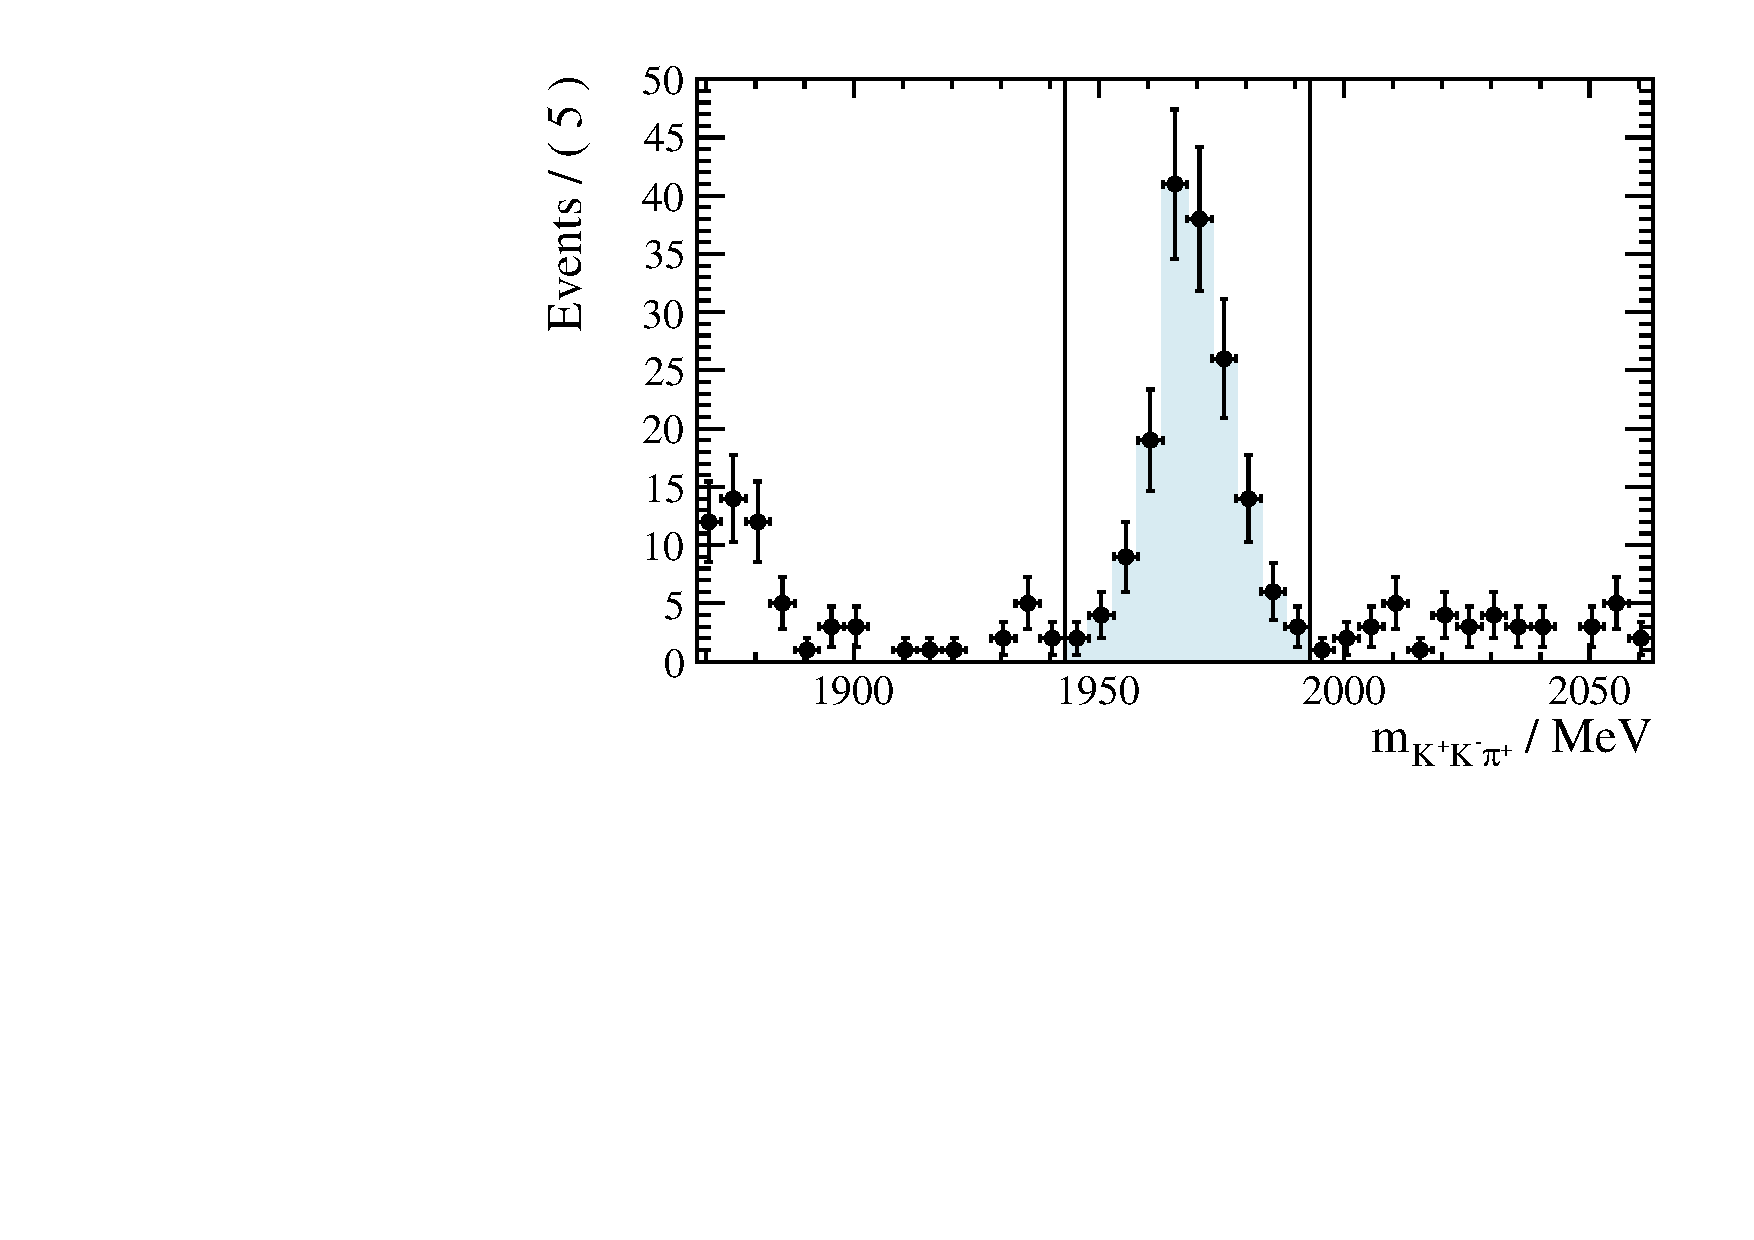
\includegraphics[width=0.48\textwidth]{spectrum_ds}
    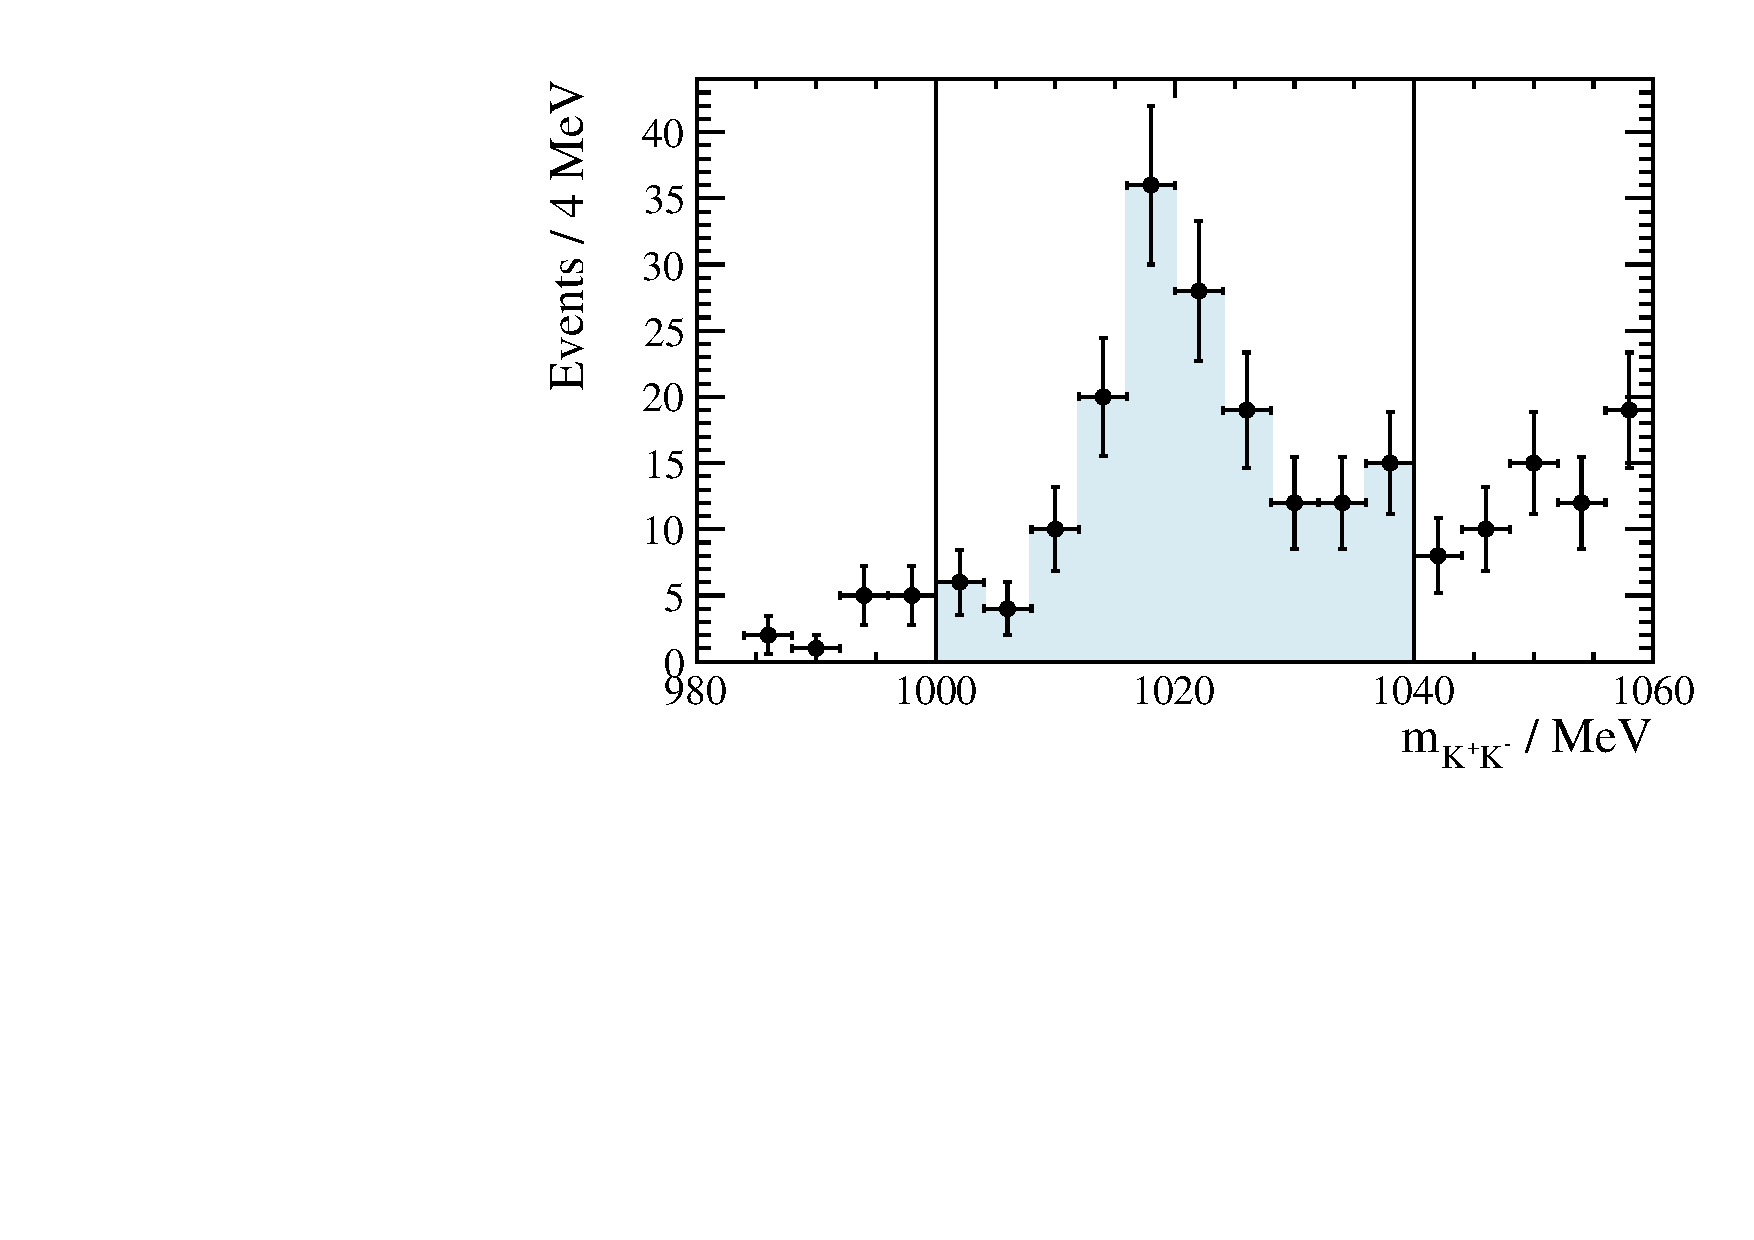
\includegraphics[width=0.48\textwidth]{spectrum_phi}
    \caption[Selected \Ds and \phii candidates]
    {
      Invariant mass distributions of the candidate
      (left) \decay{\Ds}{\kkpi}, and
      (right) \decay{\phii}{\kk} candidates.
      The \kkpi spectrum shows a range of masses, where the vertical black lines indicate the
      boundaries of the mass cut $|m_{\kkpi}-m_{\Ds}^\pdg|<25\mev$, where the shaded candidates are
      those that are accepted.
      On the far left of this distribution, a mass peak from \decay{\Dp}{\kkpi} is also visible.
      The \decay{\phi}{\kk} spectrum is shown in the range $|m_{\kk}-m_{\phi}^\pdg|<40\mev$,
      and the signal region is indicated by the vertical black lines and shaded data.
    }
    \label{fig:dsphi:mesons}
  \end{center}
\end{figure}


%\section{Results}







%\begin{equation}
  %A_\mathrm{CP}^\mathrm{obs} =
  %\frac{
    %N(\decay{\Bm}{\Dsm\phi}) - N(\decay{\Bp}{\Dsp\phi})
  %}{
    %N(\decay{\Bm}{\Dsm\phi}) + N(\decay{\Bp}{\Dsp\phi} - N_\mathrm{bkg})
  %}
%%\end{equation}

\clearpage




%So, a lot of this comes from the ANA and PAPER.
%
%
%\begin{figure}
  %\begin{center}
    %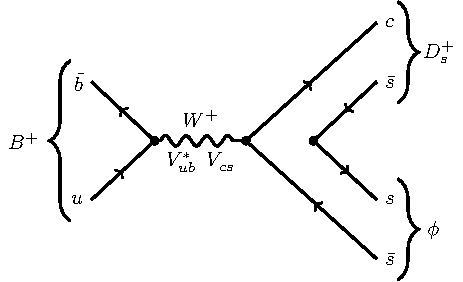
\includegraphics[scale=1]{feynman_dsphi_sm}
    %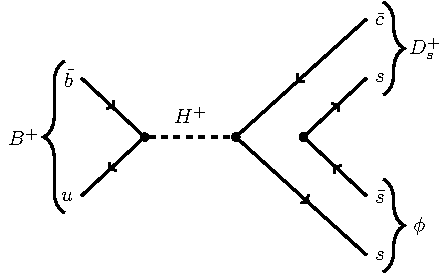
\includegraphics[scale=1]{feynman_dsphi_susy}
  %\end{center}
  %\caption[Feynman diagrams for \btodsphi in SM and BSM]
  %{\small
    %Feynman diagrams
  %}
%\end{figure}
%
%\section{Motivation}
%\begin{itemize}
  %\item First observation, fully hadronic B decay
  %\item CPV in this sector
  %\item Feynmann diagram
%\end{itemize}
%
%
%\section{Theory specific to \btodsphi}
%\begin{itemize}
  %\item CPV again, SUSY
%\end{itemize}
%
%
%\section{Data sample}
%
%
%\section{Selection}
%
%
%\subsection{Multivariate selection --- BDTs}
%\begin{itemize}
  %\item Widely used in (modern) particle physics
  %\item Basic principles
%\end{itemize}
%
%\section{Backgrounds}
%\begin{itemize}
  %\item Combinatorics (define)
  %\item All the specific peaking backgrounds
%\end{itemize}
%
%\section{Results}

